\documentclass[12pt]{article}
\title{Dokumentacja implementacji algorytmu wstecznej propagacji na przykładzie funkcji NXoR}
\author{Michał Korniak}
\date{}
\usepackage{graphicx}
\usepackage{graphics}
\usepackage[polish]{babel}
\usepackage[T1]{fontenc}
\newcommand{\source}[1]{{\centerline{\tiny Źródło: #1}}}

\usepackage{color}
\definecolor{bluekeywords}{rgb}{0.13,0.13,1}
\definecolor{greencomments}{rgb}{0,0.5,0}
\definecolor{redstrings}{rgb}{0.9,0,0}

\usepackage{listings}
\lstset{language=[Sharp]C,
  showspaces=false,
  showtabs=false,
  breaklines=true,
  showstringspaces=false,
  breakatwhitespace=true,
  escapeinside={(*@}{@*)},
  commentstyle=\color{greencomments},
  keywordstyle=\color{bluekeywords},
  stringstyle=\color{redstrings},
  basicstyle=\footnotesize,
  numbers=left,
  xleftmargin=5.0ex,
}
 


\begin{document}
\maketitle
\tableofcontents{}
\newpage


\section{Wprowadzenie}
Algorytm wstecznej propagacji błędu jest metodą uczenia wielowarstwowych polegającą na korekcie wag połączeń między neuronami na podstawie błędu całej sieci.
W tym dokumencie prześledzę działanie tego algorytmu na przykładzie nauczanie działania funkcji NXoR.
jednocześnie przedstawiając jego autorską implementację w języku C\#. 

\section{Architektura sieci dla funkcji NXoR}
Algorytm wstecznej propagacji jest wykorzystywany do nauczania wielowarstwowych sieci jednokierunkowych.
Taka sieć zawiera warstwę wejściową i warstwę wyjściową,
może posiadać również warstwy ukryte (wykorzystywana do problemów liniowo nieseparowalnych).
Każda warstwa zawiera dowolną ilość neuronów.
Neurony są połączone ze sobą w taki sposób, że każdy neuron warstwy innej niż wyjściowa jest połączony z każdym neuronem kolejnej warstwy,
a każde połączenie ma określoną wagę.
Dodatkowo możliwe jest połączenie do tego zwanego biasa, czyli połączenia do neuronu, który zawsze przyjmuje wartość 1.
Połączenia wejściowe do neuronu będą wpływać na to jaką będzie miał wartość.

Kluczowym pytaniem jest to jak powinna wyglądać sieć obsługująca funkcję NXoR. 
Jako, że funkcja ta przyjmuje dwie liczby wejściu jasne jest, że powinna posiadać również dwa neurony wejściowe.
Wiemy również, że sieć posiada jedno wyjście, co sprawia, że potrzebujemy tylko jednego neuronu wyjściowego.

\begin{center}
  \begin{tabular}{||c c c||} 
  \hline
  x1 & x2 & NXoR \\ [0.5ex] 
  \hline\hline
  0 & 0 & 1\\ 
  \hline
  0 & 1 & 0 \\
  \hline
  1 & 0 & 0 \\
  \hline
  1 & 1 & 1 \\ [0.5ex] 
  \hline
 \end{tabular}
 \end{center}
 
W powyższym opisie pojawiła się wzmianka o tym, że warstwa ukryta jest wykorzystywana w problemach, które nie są liniowo separowalne.
W związku z tym należy się zastanowić czy problem NXoR do takowych należy.
Aby sprawdzić czy problem jest liniowo separowalny należy narysować na płaszczyźnie punkty w których funkcja przyjmuje 0 i tych w których przyjmuje 1, a następnie sprawdzić czy istnieje prosta, która przedzieli te punkty na dwie płaszczyzny.
Jak pokazuje rysunek \ref{fig:separability} do funkcji spełniających ten warunek należą funkcje AND i OR.
Natomiast przykładem funkcji niespełniającej tego warunku jest XOR, a więc też jego odwrotność czyli NXoR.
W związku z tym będziemy potrzebować warstwy ukrytej.
 
\begin{figure}[!ht]
  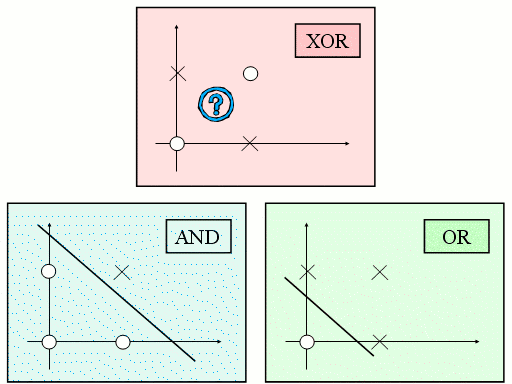
\includegraphics[width=\linewidth]{images/andorxor.png}
  \source{https://edux.pjwstk.edu.pl/mat/2144/lec/rW2.htm/}
  \caption{Liniowa separowalność funkcji AND, OR, XOR}
  \label{fig:separability}
\end{figure}

Otwartym pytaniem pozostaje natomiast to ile neuronów powinna posiadać ta warstwa.
Tutaj posłużymy się cytatem z książki Jeffa Heatona "Introduction to Neural Networks for C\#":
\begin{quote}
  There are many rule-of-thumb methods for determining the correct number of neurons to use in the hidden layers, such as the following:
  \begin{itemize}
    \item  The number of hidden neurons should be between the size of the input layer and the size of the output layer.  
    \item   The number of hidden neurons should be 2/3 the size of the input layer, plus the size of the output layer.
    \item   The number of hidden neurons should be less than twice the size of the input layer.
  \end{itemize}
\end{quote}

W związku z powyższym nasza warstwa ukryta będzie zawierała 2 neurony.

Kolejnym pytaniem jest to czy należy wprowadzać biasa.
Wstępne testy pokazały, że jego obecność przyśpiesza trening sieci,
ale aby nie komplikować opisu zostanie on pominięty.

Ostatecznie nasza sieć będzie wyglądała tak jak na rysunku \ref{fig:architecture}

\begin{figure}[!ht]
  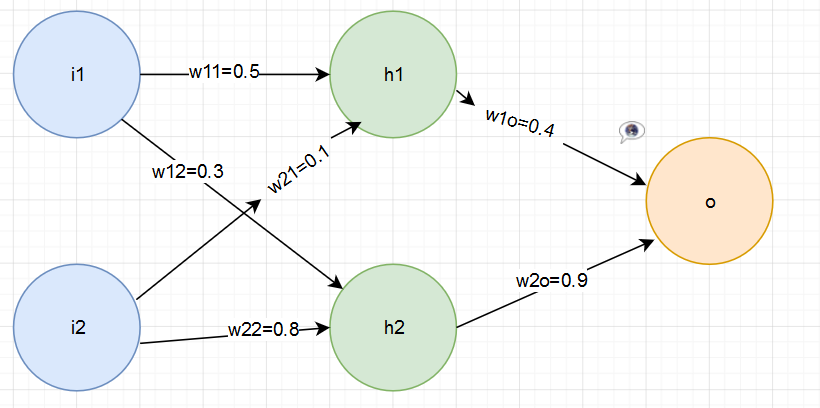
\includegraphics[width=\linewidth]{images/architecture.png}
  \caption{Architektura sieci realizującej funkcję NXoR}
  \label{fig:architecture}
\end{figure}

 


\section{Obliczanie wyjść sieci neuronowej}
Nieodzownym krokiem treningu sieci neuronowej jest obliczenie aktualnych wyników i porównanie ich z oczekiwanymi.
Przedstawmy to na przykładzie wejścia (0,1), którego oczekiwanym wyjściem jest 0.
Informację o wejściu podajemy neuronom wejściowym, tak więc:\(i1=0\), \(i2=1\).

Aby obliczyć wartości kolejnych neuronów musimy zsumować wartości połączeń do tego neuronu, a następnie poddając wynik funkcji aktywacji.
Przez wartość połączenia będziemy rozumieli iloczyn wagi i neuronu wejściowego dla połączenia.
Wagi połączeń zostały przedstawione na rysunku \ref{fig:separability}.

Przykładowo dla neuronu h1 wartość przed użyciem funkcji aktywacji będzie równa:
\[
  net_{h1}  = i1*w11+i2*w21
\]
Co po podstawieniu wartości da:
\[
  net_{h1} = 0*0.5+1*0.1=0.1
\]
Taka wartość jest następnie poddawana działaniu funkcji aktywacji, 
co umożliwia normalizowanie wartości neuronów do oczekiwanych przedziałów wartości.
W tym przypadku skorzystamy z funkcji sigmoidalnej, której zakres wartości mieści się w przedziale [0,1]:
\[
    f(x) =  \frac{1}{1 + e^{-x} } 
\]
Po podstawieniu otrzymanej wcześniej wartości do funkcji dostaniemy wartość neuronu h1:
\[
    out_{h1} 
    = f(net_{h1}) 
    =  \frac{1 }{1 + e^{-net_{h1}} } 
    =  \frac{1 }{1 + e^{-0.1} } \approx 0.525
\]
W ten sposób będziemy liczyć wartość kolejnych neuronów:
\[
    out_{h2}=f(i1*w12+i2*w22)=f(0*0.3+1*0.8)=f(0.8) \approx 0.690
\]
\[
    out_{o}=f(h1*w1o+h2*w2o)=f(0.525*0.4+0.690*0.9)=f(0.831) \approx 0.697
\]
 

% \section{Implementacja wielowarstwowej sieci neuronowej}
% 
\subsection{Tworzenie obiektu odpowiadającego sieci neuronowej}

Teraz przedstawię autorską implementację przedstawionego wcześniej algorytmu.
Podstawą jest klasa odwzorowującej sieć neuronową, w moim przypadku
taką funkcję pełni klasa NeuralNetwork, która to implementuje interfejs pokazany na listingu \ref{lst:INeuralNetwork}.

\begin{lstlisting}[caption={Interfejs INeuralNetwork}, label={lst:INeuralNetwork}]
  public interface INeuralNetwork
  {
      IEnumerable<IInputNeuron> InputLayer { get; }
      IEnumerable<IHiddenNeuron> HiddenLayer { get; }
      IEnumerable<IOutputNeuron> OutputLayer { get; }
      IErrorFunction ErrorFunction { get; }
      void FillInputNeurons(IEnumerable<double> input);
      IEnumerable<double> CalculateOutput();
  }
\end{lstlisting}

W tym momencie skupmy się na linijkach 3, 4 i 5, które to wskazują na to, że sieć neuronowa zawiera warstwy wejściową, ukrytą i wyjściową.
Jak widzimy każda warstwa posiada inny typ neuronu, co wynika to z tego, że w zależności od warstwy neurony się różnią. Przykładowo:
\begin{itemize}
  \item Neuron warstwy wejściowej nie ma możliwości dodawanie połączeń wejściowych.
  \item Neuron warstwy wyjściowej nie ma możliwości dodawanie połączeń wyjściowych.
  \item Neuron warstwy ukrytej ma możliwość dodawanie obu typów połączeń.
\end{itemize}

Obiekt klasy NeuralNetwork jest tworzony z wykorzystaniem wzorca "Builder".
Dzieje się to w sposób pokazany na listingu \ref{lst:NeuralNetworkBuilder}.

\begin{lstlisting} [caption={Budowanie obiektu NeuralNetwork},label={lst:NeuralNetworkBuilder}]
  var neuralNetworkBuilder = new NeuralNetworkBuilder();
  var network = neuralNetworkBuilder
      .SetNumberOfInputNeurons(2)
      .SetNumberOfOutputNeurons(1)
      .SetActivationFunction(new SigmoidActivationFunction())
      .SetErrorFunction(new MeanSquaredErrorFunction(1))
      .SetNumberOfHiddenNeurons(2)  //opcjonalne
      //.AddBiasConnections()         //opcjonalne
      .Build();
\end{lstlisting}

Klasa NeuralNetworkBuilder umożliwia stworzenie sieci neuronowej:
\begin{itemize}
  \item Zawierającą wybraną ilość neuronów warstwy wejściowej.
  \item Zawierającą wybraną ilość neuronów warstwy wyjściowej
  \item Działającą na określonej funkcji aktywacji
  \item Wyliczającej błąd na podstawie wybranej funkcji
  \item Umożliwiającej opcjonalne dodanie warstwy ukrytej
  \item Umożliwiającej opcjonalne dodanie połączeń do biasów
\end{itemize}

Zadaniem Buildera jest stworzenie obiektu klasy NeuralNetwork, który spełni podane wymagania. 
W zależności od tego czy użytkownik będzie potrzebował warstwy ukrytej, Builder utworzy sieć która ma połączenia z warstwą pośrednią lub też bezpośrednie połączenia warstwy wejściowej z wyjściową.
Podobnie jest z wyborem tego czy czy powinny być tworzone biasy czy też nie.
Builder nie posiada żadnej metody dotyczącej wyboru pierwotnych wag połączeń, co wynika z tego, że zgodnie z założeniem algorytmu wstecznej propagacji są one inicjalizowane losowo.

Dla tak stworzonej sieci neuronowej możemy przeprowadzić obliczenia, które zostały przedstawione w poprzednim podrozdziale.
Robimy to w sposób przedstawiony w listingu \ref{lst:CalculateOutput}

\begin{lstlisting} [caption={Budowanie obiektu NeuralNetwork},label={lst:CalculateOutput}]
  network.FillInputNeurons(new double[] { 0, 1 });
  var output = network.CalculateOutput();
\end{lstlisting}

W pierwszej kolejności są wypełniane neurony wejściowe.
Jeśli użytkownik poda liczbę danych wejściowych różniącą się od liczby neuronów warstwy wejściowej zostanie wyrzucony wyjątek.

Wyjście sieci jest liczone w sposób rekurencyjny:
\begin{itemize}
  \item Wyjście każdego neuronu z wyjątkiem neuronów wejściowych jest sumą wyjść połączeń wejściowych poddanych funkcji aktywacji (listing \ref{lst:NeuronOutput}).
  \item Wyjście połączenia jest iloczynem wagi i wyjścia neuronu źródłowego (listing \ref{lst:ConnectionOutput})
\end{itemize}

\begin{lstlisting} [caption={Wyliczanie wyjścia neuronu},label={lst:NeuronOutput}]
  public class OutputNeuron : IOutputNeuron
  {
      //***
      public double NetOutput => _inputConnections.Sum(x => x.Output);
      public double Output => _activationFunction.Invoke(NetOutput);
      //***
  }
\end{lstlisting}


\begin{lstlisting} [caption={Wyliczanie wyjścia połączenia},label={lst:ConnectionOutput}]
  class NeuronConnection: INeuronConnection
  {
      //***
      public double Output => Weight * _source.Output;
      //***
  }
\end{lstlisting}

\subsection{Implementacja treningu sieci neuronowej}

Aby rozpocząć proces uczenia należy stworzyć instancję klasy Trainer, która to przyjmuje w konstruktorze
informację na temat sieci, którą będziemy chcieli uczyć oraz stałej uczenia. 
Kolejnym krokiem jest przygotowanie danych testowych, na podstawie których nauczymy naszą sieć określonych zachowań.
Następnie należy wywołać funkcję Train, przekazując jej kolekcję danych testowych oraz warunki stopu,
to znaczy maksymalną liczbę epok po których nauczanie się zatrzyma oraz błąd po którego osiągnięciu nauczanie zostanie zakończone.
Cała ta procedura została pokazana na listingu \ref{lst:train-invoke}.


\begin{lstlisting} [caption={Rozpoczęcie procesu uczenia },label={lst:train-invoke}]
  var trainer = new Trainer(neuralNetwork: network, learningRate: 0.01, logger: new ConsoleLogger());
  var trainDataCollection = new[]
  {
      new TrainData(new double []{ 0, 0 },new double [] { 1 } ),
      new TrainData(new double []{ 1, 0 },new double [] { 0 } ),
      new TrainData(new double []{ 0, 1 },new double [] { 0 } ),
      new TrainData(new double []{ 1, 1 },new double [] { 1 } ),
  };
  trainer.Train(trainDataCollection, numberOfEpochs: 1000000, terminalEpochError:0.01);
\end{lstlisting}

Sama funkcja Train steruje przebiegiem uczenia (listing \ref{lst:train-invoke})
W pierwszej kolejności wywołuje funkcję odpowiedzialną za sprawdzenie tego czy w danych testowych liczba danych na wejściu oraz na wyjściu zgadza się z liczbą neuronów w odpowiednich warstwach.
Jeśli ten warunek jest spełniony funkcja wywołuje w pętli metodę TrainForSingleEpoch do czasu aż zostanie spełniony którykolwiek warunek stopu.

\begin{lstlisting} [caption={Funkcja Train},label={lst:train-function}]
  public void Train(TrainData[] trainDataCollection, int numberOfEpochs, double terminalEpochError)
  {
    ValidateTrainData(trainDataCollection);

    int i;
    double epochError = -1;
    var stopwatch = new Stopwatch();
    stopwatch.Start();
    for (i = 0; i < numberOfEpochs; ++i)
    {
        epochError = TrainForSingleEpoch(trainDataCollection);
        _logger.Info($"Epoch {i + 1}, error: {epochError}");
        _logger.Trace("___________________");
        if (epochError <= terminalEpochError)
        {
            break;
        }
    }
    stopwatch.Stop();

    return new TrainStats(i, epochError, (double)stopwatch.ElapsedMilliseconds / 1000);
  }
\end{lstlisting}

Funkcja TrainForSingleEpoch (listing \ref{lst:TrainForSingleEpoch-function}) iteruje po danych testowych wewnątrz jednej epoki wywołując na nich szereg funkcji.
Pierwszą z nich jest ta wypełniająca sieć danymi testowymi na wejściu (linia 6). Dzięki tej operacji jesteśmy w stanie obliczyć wyjście sieci co umożliwia skorzystanie z dwóch kolejnych funkcji.
Funkcja HandleOutputLayer jest w stanie obliczyć błąd średniokwadratowy między wartością oczekiwaną a rzeczywistą oraz współczynnik delta.
Współczynnik ten będzie przydatny przy liczeniu nowych wag zgodnie z opisem z poprzedniego rozdziału.
W przypadku funkcji HandleHiddenLayer liczymy wartość delty dla neuronów warstwy ukrytej.


\begin{lstlisting} [caption={Funkcja TrainForSingleEpoch},label={lst:TrainForSingleEpoch-function}]
  private double TrainForSingleEpoch(TrainData[] trainDataCollection)
  {
    double totalEpochError = 0;
    foreach (var trainData in trainDataCollection)
    {
        _logger.Trace("");
        _logger.Trace($"Input: ({string.Join(",", trainData.Inputs)})");
        _network.FillInputNeurons(trainData.Inputs);
        HandleOutputLayer(trainData.ExpectedOutputs);
        _logger.Trace($"Output: ({string.Join(",", _network.OutputLayer.Select(x => x.Output))})");
        _logger.Trace($"Expected: ({string.Join(",", trainData.ExpectedOutputs)})");
        HandleHiddenLayer();
        UpdateWeights();
        double iterationError = _network.OutputLayer.Sum(x => x.Error);
        _logger.Trace($"Iteration error: {iterationError}");
        totalEpochError += iterationError;
    }
    _logger.Trace("");
    return totalEpochError;
  }

  private void HandleOutputLayer(double[] expectedOutputs)
  {
      for (int i = 0; i < expectedOutputs.Length; ++i)
      {
          var outputNeuron = _network.OutputLayer.ElementAt(i);
          var expectedOutput = expectedOutputs[i];

          outputNeuron.CalculateError(_network.ErrorFunction, expectedOutput);
          outputNeuron.CalculateDeltaError(_network.ErrorFunction, expectedOutput);
      }
  }
  private void HandleHiddenLayer()
  {
      foreach (var hiddenNeuron in _network.HiddenLayer)
      {
          hiddenNeuron.CalculateDeltaError();
      }
  }

\end{lstlisting}

Funkcja UpdateWeights iteruje po wszystkich połączeniach wywołując na nich funkcje aktualizujące wagi.
W przypadku połączeń między neuronami wywoływana jest funkcja przedstawiona w listingu \ref{lst:UpdateNeuronConnectionWeight-function}.
Funkcja ta korzysta ze wzoru, który wynika z obliczeń przedstawionym w podrozdziale dotyczącym korygowania wag:
\[
w^+=w-\eta*\frac{\partial E_{total}}{\partial w}  
\]
gdzie:
\[
  \frac{\partial E_{total}}{\partial w}  =\delta_{output}*input
\]

\begin{lstlisting} [caption={Funkcja TrainForSingleEpoch},label={lst:UpdateNeuronConnectionWeight-function}]
private void UpdateNeuronConnectionWeight(INeuronConnection neuronConnection)
{
    var destinationNeuron = neuronConnection.Destination as INeuronWithDeltaError;
    var derivatateOfTotalErrorToWeight = neuronConnection.Input * destinationNeuron.DeltaError;
    neuronConnection.Weight -= _learningRate * derivatateOfTotalErrorToWeight;
}
\end{lstlisting}

\subsection{Badanie mające na celu wyszukanie najlepszej architektury sieci realizującej funkcję NXOR}

Jak pokazuje listing \ref{lst:train-function} po każdym treningu są zwracane informacje na temat statystyk 
procesu nauczania. Są to:
\begin{itemize}
  \item błąd całkowity dla danych testowych w ostatnim treningu epoki
  \item liczba epok wykonanych w ramach treningu
  \item czas potrzebny na wykonanie treningu
\end{itemize}

Dzięki tym informacjom jesteśmy w stanie przeprowadzić test mający na celu wyszukanie najlepszej architektury
sieci neuronowej realizującej funkcję NXOR.
Jak wiadomo sieć sieć realizująca taka funkcję musi mieć dwa neurony wejściowe oraz jeden wyjściowy,
natomiast kwestią którą będziemy chcieli ustalić jest ilość neuronów ukrytych oraz to
czy warto stworzyć połączenia do biasa.

Aby dowiedzieć się jaka architektura będzie najbardziej optymalna przeprowadzono po 100 testów
dla sieci posiadających od 1 do 5 neuronów w warstwie ukrytej, posiadającej lub nie posiadającej połączenia
do biasa (Klasa Runner.ArchitectureTest.UnipolarNXORArchitectureTest).
Każdy test miał ustawione warunki stopu na 100000 epok lub błąd całkowity równy 0.1.
Następnie zostały porównane mediany dla danych konfiguracji. Oto wyniki:

\begin{scriptsize}  
  Number of neurons in hidden layer: 1
  Bias: NO
  Median results:
  Number of epochs: 100000, average error: 1,00020034941792, elapsed time: 6,905 seconds
  
  Number of neurons in hidden layer: 2
  Bias: NO
  Median results:
  Number of epochs: 100000, average error: 0,3239291988340041, elapsed time: 10,706 seconds
  
  Number of neurons in hidden layer: 3
  Bias: NO
  Median results:
  Number of epochs: 64608, average error: 0,09999773905181816, elapsed time: 8,265 seconds
  
  Number of neurons in hidden layer: 4
  Bias: NO
  Median results:
  Number of epochs: 59230, average error: 0,09999703805996166, elapsed time: 8,445 seconds
  
  Number of neurons in hidden layer: 5
  Bias: NO
  Median results:
  Number of epochs: 59027, average error: 0,09999687258536925, elapsed time: 10,545 seconds
  
  Number of neurons in hidden layer: 1
  Bias: YES
  Median results:
  Number of epochs: 100000, average error: 0,6852163896622288, elapsed time: 11,749 seconds
  
  Number of neurons in hidden layer: 2
  Bias: YES
  Median results:
  Number of epochs: 60466, average error: 0,09999632349029491, elapsed time: 10,212 seconds
  
  Number of neurons in hidden layer: 3
  Bias: YES
  Median results:
  Number of epochs: 49232, average error: 0,09999588993519329, elapsed time: 10,477 seconds
  
  Number of neurons in hidden layer: 4
  Bias: YES
  Median results:
  Number of epochs: 47013, average error: 0,09999732020772159, elapsed time: 12,965 seconds
  
  Number of neurons in hidden layer: 5
  Bias: YES
  Median results:
  Number of epochs: 60467, average error: 0,09999979050186819, elapsed time: 15,098 seconds
  
\end{scriptsize}

Jak widać sieć osiąga oczekiwany błąd całkowity aż w 7 konfiguracjach.
Ten cel został osiągnięty w najmniejszej liczbie epok w przypadku dla 4 neuronów z biasem.
Jednakże pomimo tego ten przypadek jest dość mało wydajny jeśli spojrzymy na czas, 
gdyż jest on prawie o 5 sekund wolniejszy od najszybszego przypadku z 3 neuronami bez biasa.
Wynika to z tego, że każde dodatkowe połączenie wymaga dodatkowych obliczeń,
co sprawia, że powinniśmy ostrożnie zwiększać ich ilość w naszych sieciach. 


\section{Trening sieci neuronowej}
Jak widzimy otrzymany wynik różni się od oczekiwanego.
Dlatego też przeprowadzimy trening sieci, którego celem będzie ustawienie wag w ten sposób,
żeby wyjście sieci jak najbardziej odpowiadało wartości oczekiwanej.

Mając obliczone wyjście sieci oraz wartością oczekiwaną możemy obliczyć wartość błędu.
Robimy to przy pomocy funkcji błędu średniokwadratowego.

\[
    E(O)=1/n*(d-o)^2
\]
gdzie:
\begin{itemize}
  \item E(O) to błąd średniokwadratowy dla konkretnego neuronu wyjściowego
  \item n to liczba neuronów warstwy wyjściowej
  \item d to oczekiwane wyjście neuronu
  \item o to rzeczywiste wyjście neuronu
\end{itemize}

Dla sieci z rysunku \ref{fig:architecture} i wejścia (0,1) wartość jedynego neuronu wyjściowego jest równa 0.697. 
Natomiast jego wartość oczekiwana to 1. W związku z tym błąd średniokwadratowy jest równy:

\[
    E_{o} = 1/1 * (1-0.697)^2 \approx 0.092
\]


Naszym celem będzie takie ustawienie wag,
aby jak najbardziej zminimalizować błąd. Robimy to za pomocą wzoru:

\begin{gather}
  \begin{aligned}
  w^{+} = w - \eta * \frac{\partial E_{total}}{\partial w}\\
  \end{aligned}\notag
  \shortintertext{gdzie:}
  \begin{aligned}
    &w^{+} ~\text{jest nową wartością wagi}.\\
    &w ~\text{jest aktualną wartością wagi}.\\
    &\eta ~\text{jest stałą uczenia, czyli wartością, która określa szybkość uczenia sieci}.\\
    &\frac{\partial E_{total}}{\partial w} ~\text{jest pochodną częściową błędu całkowitego sieci do danej wagi.}
  \end{aligned}\notag
\end{gather}

Szczególną uwagę należy poświecić stałej uczenia \texteta.
Jest ona ustawiana w momencie rozpoczynania procesu, przyjmując wartości z zakresu [0,1].
W zależności od wybranej wartości zmiany wag będą postępować gwałtowanie lub też łagodnie. 
Zazwyczaj stała uczenia jest ustawiane na wartości mniejsze bądź równe 0.1.
W naszym przypadku będzie to 0.1.

Kolejną rzeczą wartą uwagi jest pochodna błędu całkowitego do konkretnej wagi.
Liczymy ją z wykorzystaniem reguły łańcuchowej, w przypadku w1o:
\[
  \frac{\partial E_{total}}{\partial w1o} = \frac{\partial E_{total}}{\partial out_{o}} * \frac{\partial out_{o}}{\partial net_{o}} * \frac{\partial net_{o}}{\partial w1o}
\]
Już teraz możemy zauważyć, że wzór na pochodną cząstkową dla w2o będzie bardzo podobny:
\[
  \frac{\partial E_{total}}{\partial w2o} = \frac{\partial E_{total}}{\partial out_{o}} * \frac{\partial out_{o}}{\partial net_{o}} * \frac{\partial net_{o}}{\partial w2o}
\]

Wynika to z tego, że oba połączenie mają taki neuron docelowy.
Aby nie liczyć tego samego dwa razy, możemy wprowadzić oznaczenie dla części wspólnej równania:
\[
  \delta_{o} = \frac{\partial E_{total}}{\partial net_{o}} = \frac{\partial E_{total}}{\partial out_{o}} * \frac{\partial out_{o}}{\partial net_{o}} 
\]
tym samym:
\[
  \frac{\partial E_{total}}{\partial w1o} = \delta_{o}  * \frac{\partial net_{o}}{\partial w1o}
\]
\[
  \frac{\partial E_{total}}{\partial w2o} = \delta_{o}  * \frac{\partial net_{o}}{\partial w2o}
\]

Spróbujmy teraz uprościć wyrażenie \(\frac{\partial net_{o}}{\partial w1o}\):
\[
  \frac{\partial net_{o}}{\partial w1o} = \frac{\partial (w1o * out_{h1} + w2o * out_{h2})}{\partial w1o}
  = 1 * out_{h1} * w1o^{(1 - 1)} + 0 + 0 = out_{h1}
\]
Jak widzimy \(\frac{\partial net_{o}}{\partial w1o}\) ostatecznie sprowadza się do wartości neuronu źródłowego dla połączenia.
W analogiczny sposób upraszcza się równanie dla \(\frac{\partial net_{o}}{\partial w2o}\), dzięki czemu otrzymujemy:
\[
  \frac{\partial E_{total}}{\partial w1o} = \delta_{o}  * out_{h1}
\]
\[
  \frac{\partial E_{total}}{\partial w2o} = \delta_{o}  * out_{h2}
\]

Ostatnim krokiem potrzebnym do wyliczenia nowych wag jest obliczenie samego współczynnika delty dla \(o_1\) (\(\delta_{o}\)):

\[
  \delta_{o} = \frac{\partial E_{total}}{\partial net_{o}} = \frac{\partial E_{total}}{\partial out_{o}} * \frac{\partial out_{o}}{\partial net_{o}}
\]

\[
  \frac{\partial E_{total}}{\partial out_{o}} = \frac{\partial (d_{o} - out_{o})^{2}}{\partial out_{o}}= -(target_{o} - out_{o})
\]


\begin{gather}
  \begin{aligned}
    &\frac{\partial out_{o}}{\partial net_{o}} =  \frac{\partial (\frac{1}{1+e^{-net_{o}}})}{\partial net_{o}}=({\frac{1}{1+e^{-net_{o}}})}(1 - \frac{1}{1+e^{-net_{o}}})
  \end{aligned}\\
  \shortintertext{gdzie:}
  \begin{aligned}
    \frac{1}{1+e^{-net_{o}}}=out_o
  \end{aligned}
  \shortintertext{a więc:}
  \begin{aligned}
    \frac{\partial out_{o}}{\partial net_{o}} = out_{o}(1 - out_{o})
  \end{aligned}
\end{gather}

W związku z powyższymi równaniami wzór na współczynnik delty dla \(out_o\) wynosi:

\[
  \delta_{o} =\frac{\partial E_{total}}{\partial net_{o}} = \frac{\partial E_{total}}{\partial out_{o}} * \frac{\partial out_{o}}{\partial net_{o}}=-(target_{o} - out_{o}) * out_{o}(1 - out_{o})
\]

Co podstawieniu daje:
\[
  \delta_{o} \approx -0.064
\]

W ten sposób otrzymaliśmy łatwy wzór na obliczenie pochodnych cząstkowej po w1o i w2o
\[
  \frac{\partial E_{total}}{\partial w1o} = \delta_{o}  * out_{h1} \approx  -0.064 * 0.525 \approx -0.0336
\]
\[
  \frac{\partial E_{total}}{\partial w2o} = \delta_{o}  * out_{h2} \approx  -0.064 * 0.690 \approx -0.04416
\]

co umożliwia nam obliczenie nowych wag:
\[
  w1o^{+} = w1o - \eta * \frac{\partial E_{total}}{\partial w1o} = 0.4 - 0.1 * -0.0336 = 0.40336 
\]
\[
  w2o^{+} = w2o - \eta * \frac{\partial E_{total}}{\partial w2o} = 0.9 - 0.1 * -0.04416 = 0.904416
\]

Spróbujmy teraz ustalić jakie wartości powinny przyjąć wagi połączeń pomiędzy warstwą wejściową a warstwą ukrytą.
Stosujemy tutaj ten sam wzór co do połączeń pomiędzy warstwą ukrytą a warstwą wyjściową, tak więc wzór na wagę w11 będzie wyglądał tak:
\[
  w11^{+} = w11 - \eta * \frac{\partial E_{total}}{\partial w11}
\]

Tak jak poprzednio najbardziej problematyczne będzie wyznaczenie pochodnej błędu całkowitego do tej wagi:
\[
  \frac{\partial E_{total}}{\partial w11}=
  \frac{\partial E_{total}}{\partial out_{o1}}*
  \frac{\partial out_{o1}}{\partial net_{o1}}*
  \frac{\partial net_{o1}}{\partial out_{h1}}*
  \frac{\partial out_{h1}}{\partial net_{h1}}*
  \frac{\partial net_{h1}}{\partial w11}
\]
Od razu zauważmy, że pochodna błędu całkowitego do wagi drugiego połączenia (w21) do tego neuronu jest bardzo podobna:
\[
  \frac{\partial E_{total}}{\partial w21}=
  \frac{\partial E_{total}}{\partial out_{o1}}*
  \frac{\partial out_{o1}}{\partial net_{o1}}*
  \frac{\partial net_{o1}}{\partial out_{h1}}*
  \frac{\partial out_{h1}}{\partial net_{h1}}*
  \frac{\partial net_{h1}}{\partial w21}
\]

Podobnie jak w przypadku neuronów wyjściowych oznaczmy część wspólną tych równań jako \(\delta h1\):
\[
  \delta h1=
  \frac{\partial E_{total}}{\partial out_{o1}}*
  \frac{\partial out_{o1}}{\partial net_{o1}}*
  \frac{\partial net_{o1}}{\partial out_{h1}}*
  \frac{\partial out_{h1}}{\partial net_{h1}}
\]

Można jednak zauważyć, że pierwsza część równania to tak naprawdę \(\delta o\), którą mamy już wyliczoną:
\[
  \delta h1=
  \delta o *
  \frac{\partial net_{o1}}{\partial out_{h1}}*
  \frac{\partial out_{h1}}{\partial net_{h1}}*
\]

Obliczmy teraz dwie pozostałe pochodne:
\[
  \frac{\partial net_{o1}}{\partial out_{h1}} = \frac{\partial (w1o * out_{h1} + w2o * out_{h2})}{\partial out_{h1}}=w1o
\]
\[
  \frac{\partial out_{h1}}{\partial net_{h1}}= \frac{\partial out_{h1}}{\partial net_{h1}} = out_{h1}(1 - out_{h1})
\]

Tak więc ostatecznie wyznacznik delta dla neuronu h1 jest równy:
\[
  \delta h1= \delta o * w1o * out_{h1}(1 - out_{h1}) = -0.064 * 0.4 * 0.249375 = -0.006384
\]

Wiedząc, że pochodna wartości neuronu przed funkcją aktywacji po wadze jest równa wartości neuronu z którego wychodzi połączenie
możemy obliczyć również pochodne cząstkowe po wagach w11 i w21
\[
  \frac{\partial E_{total}}{\partial w11}=\delta h1 * \frac{\partial net_{h1}}{\partial w11}=\delta h1 * out_{i1}=-0.006384 * 0=0
\]
\[
  \frac{\partial E_{total}}{\partial w21}=\delta h1 * \frac{\partial net_{h1}}{\partial w21}=\delta h1 * out_{i2}=-0.006384 * 1=-0.006384
\]

Dzięki którym jesteśmy w stanie obliczyć nowe wagi w11 i w21:
\[
  w11^{+} = w11 - \eta * \frac{\partial E_{total}}{\partial w11}=0.5-0.1*0=0.5
\]
\[
  w21^{+} = w21 - \eta * \frac{\partial E_{total}}{\partial w21}=0.1-0.1*-0.006384=0.1006384
\]

W analogiczny sposób wyliczamy również wagi dla połączeń między neuronami warstwy wejściowej a neuronem h2:
\[
  w12^{+} = w12 - \eta * \frac{\partial E_{total}}{\partial w11}=w12 - \eta * \delta h2 * out_{i1}=0.3-0.1*-0.00547584*0=0.3
\]
\[
  w22^{+} = w22 - \eta * \frac{\partial E_{total}}{\partial w21}=w12 - \eta * \delta h2 * out_{i2}=0.8-0.1*-0.00547584*1=0.800547584
\]

Wielokrotne uruchomienie takiego algorytmu sprawi, że sieć będzie dawała oczekiwane rezultaty





 


\end{document}

